% What token_mask and dropout remove from a (tokens, channels) activation, and
% where the 2 named placements apply them in a block. A toy grid of 1 CLS token and
% 8 patch tokens by 12 channels stands in for ViT's 197 by 768. Compiled by render.py.
\documentclass[tikz,border=6pt]{standalone}
\usepackage[T1]{fontenc}
\usepackage{lmodern}
\usetikzlibrary{arrows.meta,positioning,calc,patterns}

\definecolor{tm}{HTML}{009E73}
\definecolor{rd}{HTML}{D55E00}
\definecolor{trig}{HTML}{CC79A7}
\definecolor{boxfill}{HTML}{F2F2F2}

\tikzset{
  op/.style={draw, rounded corners=2pt, fill=boxfill, minimum height=7mm,
    minimum width=11mm, font=\scriptsize\sffamily, align=center},
  add/.style={draw, circle, inner sep=0pt, minimum size=4mm, font=\scriptsize},
  flow/.style={-{Stealth[length=1.6mm]}, thick},
}

% \grid{x}{y}{masked rows}{masked cells}: rows are tokens (0 = CLS), columns channels.
\newcommand{\cellsize}{0.32}

\begin{document}
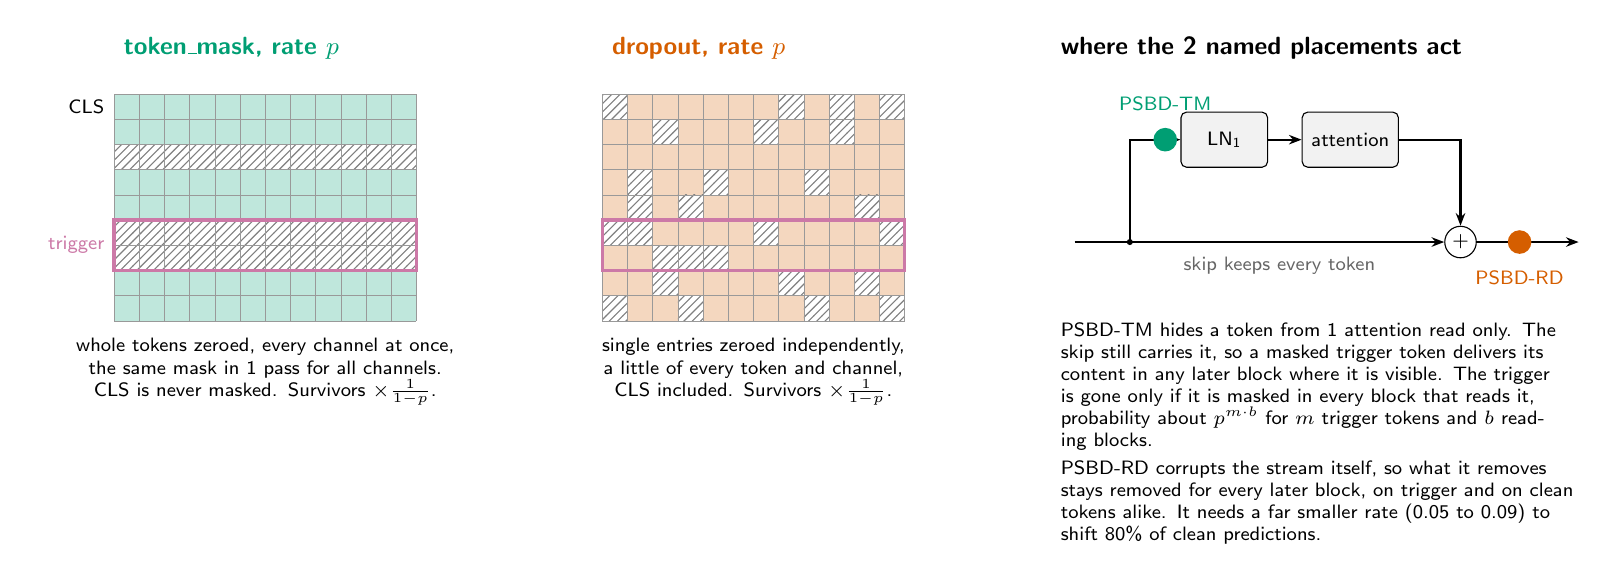
\begin{tikzpicture}

% Token mask: whole rows zeroed, CLS (row 0) protected, survivors scaled by 1/(1-p).
\begin{scope}[shift={(0,0)}]
  \node[font=\small\sffamily\bfseries, text=tm, anchor=south west] at (0, 3.2) {token\_mask, rate $p$};
  \foreach \r in {0,...,8} {
    \foreach \c in {0,...,11} {
      \pgfmathsetmacro{\y}{2.88-\r*\cellsize}
      \pgfmathsetmacro{\x}{\c*\cellsize}
      \fill[tm!25] (\x, \y) rectangle ++(\cellsize, -\cellsize);
    }
  }
  \foreach \r in {2,5,6} {
    \pgfmathsetmacro{\y}{2.88-\r*\cellsize}
    \fill[white] (0, \y) rectangle ++(12*\cellsize, -\cellsize);
    \fill[pattern=north east lines, pattern color=black!50] (0, \y) rectangle ++(12*\cellsize, -\cellsize);
  }
  \draw[step=\cellsize, black!40, very thin, shift={(0,0.0)}] (0, 2.88) grid (12*\cellsize, 2.88-9*\cellsize);
  \draw[trig, very thick] (0, 2.88-5*\cellsize) rectangle (12*\cellsize, 2.88-7*\cellsize);
  \node[font=\scriptsize\sffamily, anchor=east] at (0, 2.88-0.5*\cellsize) {CLS};
  \node[font=\scriptsize\sffamily, anchor=east, text=trig] at (0, 2.88-6*\cellsize) {trigger};
  \node[font=\scriptsize\sffamily, anchor=north, align=center, text width=58mm]
    at (6*\cellsize, -0.1) {whole tokens zeroed, every channel at once,\\the same mask in 1 pass for all channels.\\CLS is never masked. Survivors $\times\frac{1}{1-p}$.};
\end{scope}

% Dropout: independent (token, channel) entries zeroed.
\begin{scope}[shift={(6.2,0)}]
  \node[font=\small\sffamily\bfseries, text=rd, anchor=south west] at (0, 3.2) {dropout, rate $p$};
  \foreach \r in {0,...,8} {
    \foreach \c in {0,...,11} {
      \pgfmathsetmacro{\y}{2.88-\r*\cellsize}
      \pgfmathsetmacro{\x}{\c*\cellsize}
      \pgfmathtruncatemacro{\h}{mod(\r*7+\c*5+\r*\c*3, 11)}
      \ifnum\h<3
        \fill[pattern=north east lines, pattern color=black!50] (\x, \y) rectangle ++(\cellsize, -\cellsize);
      \else
        \fill[rd!25] (\x, \y) rectangle ++(\cellsize, -\cellsize);
      \fi
    }
  }
  \draw[step=\cellsize, black!40, very thin] (0, 2.88) grid (12*\cellsize, 2.88-9*\cellsize);
  \draw[trig, very thick] (0, 2.88-5*\cellsize) rectangle (12*\cellsize, 2.88-7*\cellsize);
  \node[font=\scriptsize\sffamily, anchor=north, align=center, text width=58mm]
    at (6*\cellsize, -0.1) {single entries zeroed independently,\\a little of every token and channel,\\CLS included. Survivors $\times\frac{1}{1-p}$.};
\end{scope}

% Where each is applied: PSBD-TM on the branch input, PSBD-RD on the stream.
\begin{scope}[shift={(12.2,1.0)}]
  \node[font=\small\sffamily\bfseries, anchor=south west] at (-0.3, 2.2) {where the 2 named placements act};
  \coordinate (in) at (0, 0);
  \node[op] (ln) at (1.9, 1.3) {LN\textsubscript{1}};
  \node[op] (att) at (3.5, 1.3) {attention};
  \node[add] (a) at (4.9, 0) {$+$};
  \coordinate (out) at (6.4, 0);
  \draw[flow] (in) -- (a);
  \draw[flow] (0.7, 0) |- (ln);
  \draw[flow] (ln) -- (att);
  \draw[flow] (att) -| (a);
  \draw[flow] (a) -- (out);
  \fill (0.7, 0) circle (1.1pt);
  \fill[tm] (1.15, 1.3) circle (1.5mm);
  \node[font=\scriptsize\sffamily, text=tm, anchor=south] at (1.15, 1.55) {PSBD-TM};
  \fill[rd] (5.65, 0) circle (1.5mm);
  \node[font=\scriptsize\sffamily, text=rd, anchor=north] at (5.65, -0.25) {PSBD-RD};
  \node[font=\scriptsize\sffamily, text=black!60] at (2.6, -0.3) {skip keeps every token};
  \node[font=\scriptsize\sffamily, align=left, anchor=north west, text width=66mm] at (-0.3, -0.9) {%
    PSBD-TM hides a token from 1 attention read only. The skip still carries it,
    so a masked trigger token delivers its content in any later block where it
    is visible. The trigger is gone only if it is masked in every block that
    reads it, probability about $p^{m\cdot b}$ for $m$ trigger tokens and $b$
    reading blocks.\\[2pt]
    PSBD-RD corrupts the stream itself, so what it removes stays removed for
    every later block, on trigger and on clean tokens alike. It needs a far
    smaller rate (0.05 to 0.09) to shift 80\% of clean predictions.};
\end{scope}

\end{tikzpicture}
\end{document}
